%----------------------------------------------------------------------------------------

\documentclass[a4paper,10pt]{article} % Uses article class in A4 format

%----------------------------------------------------------------------------------------
%	FORMATTING
%----------------------------------------------------------------------------------------

\setlength{\parskip}{0pt}
\setlength{\parindent}{0pt}
\setlength{\voffset}{-15pt}

%----------------------------------------------------------------------------------------
%	PACKAGES AND OTHER DOCUMENT CONFIGURATIONS
%----------------------------------------------------------------------------------------

\usepackage[a4paper, margin=2.5cm]{geometry} % Sets margin to 2.5cm for A4 Paper
\usepackage[onehalfspacing]{setspace} % Sets Spacing to 1.5

\usepackage[T1]{fontenc} % Use European encoding
\usepackage[utf8]{inputenc} % Use UTF-8 encoding
\usepackage{charter} % Use the Charter font
\usepackage{microtype} % Slightly tweak font spacing for aesthetics

\usepackage[english]{babel} % Language hyphenation and typographical rules

\usepackage{amsthm, amsmath, amssymb} % Mathematical typesetting
\usepackage{marvosym, wasysym} % More symbols
\usepackage{float} % Improved interface for floating objects
\usepackage[final, colorlinks = true, 
            linkcolor = black, 
            citecolor = black,
            urlcolor = black]{hyperref} % For hyperlinks in the PDF
\usepackage{graphicx, multicol} % Enhanced support for graphics
\usepackage{xcolor} % Driver-independent color extensions
\usepackage{rotating} % Rotation tools
\usepackage{listings, style/lstlisting} % Environment for non-formatted code, !uses style file!
\usepackage{pseudocode} % Environment for specifying algorithms in a natural way
\usepackage{style/avm} % Environment for f-structures, !uses style file!
\usepackage{booktabs} % Enhances quality of tables

\usepackage{tikz-qtree} % Easy tree drawing tool
\tikzset{every tree node/.style={align=center,anchor=north},
         level distance=2cm} % Configuration for q-trees
\usepackage{style/btree} % Configuration for b-trees and b+-trees, !uses style file!

\usepackage{titlesec} % Allows customization of titles
\renewcommand\thesection{\arabic{section}.} % Arabic numerals for the sections
\titleformat{\section}{\large}{\thesection}{1em}{}
\renewcommand\thesubsection{\alph{subsection})} % Alphabetic numerals for subsections
\titleformat{\subsection}{\large}{\thesubsection}{1em}{}
\renewcommand\thesubsubsection{\roman{subsubsection}.} % Roman numbering for subsubsections
\titleformat{\subsubsection}{\large}{\thesubsubsection}{1em}{}

\usepackage[all]{nowidow} % Removes widows

\usepackage[backend=biber,style=numeric,
            sorting=nyt, natbib=true]{biblatex} % Complete reimplementation of bibliographic facilities
\addbibresource{main.bib}
\usepackage{csquotes} % Context sensitive quotation facilities

\usepackage[yyyymmdd]{datetime} % Uses YEAR-MONTH-DAY format for dates
\renewcommand{\dateseparator}{-} % Sets dateseparator to '-'

\usepackage{fancyhdr} % Headers and footers
\pagestyle{fancy} % All pages have headers and footers
\fancyhead{}\renewcommand{\headrulewidth}{0pt} % Blank out the default header
\fancyfoot[L]{\textsc{Robin Worreby}} % Custom footer text
\fancyfoot[C]{} % Custom footer text
\fancyfoot[R]{\thepage} % Custom footer text

\newcommand{\note}[1]{\marginpar{\scriptsize \textcolor{red}{#1}}} % Enables comments in red on margin
\usepackage[shortlabels]{enumitem}
\usepackage{minted}
\usepackage[bf]{caption} 

%----------------------------------------------------------------------------------------

\begin{document}

%----------------------------------------------------------------------------------------
%	TITLE SECTION
%----------------------------------------------------------------------------------------

\title{template_assignment} % Article title
\fancyhead[C]{}
\begin{minipage}{0.295\textwidth} % Left side of title section
\raggedright
HPCSE1\\ % Your lecture or course
\footnotesize % Authors text size
%\hfill\\ % Uncomment if right minipage has more lines
Robin Worreby, 16-921-298 % Your name, your matriculation number
\medskip\hrule
\end{minipage}
\begin{minipage}{0.4\textwidth} % Center of title section
\centering 
\large % Title text size
Exercise 01\\ % Assignment title and number
\normalsize % Subtitle text size
Amdahl’s Law, Cache\\ % Assignment subtitle
\end{minipage}
\begin{minipage}{0.295\textwidth} % Right side of title section
\raggedleft
\today\\ % Date
\footnotesize % Email text size
%\hfill\\ % Uncomment if left minipage has more lines
rworreby@student.ethz.ch% Your email
\medskip\hrule
\end{minipage}

%----------------------------------------------------------------------------------------
%	ARTICLE CONTENTS
%----------------------------------------------------------------------------------------

\setcounter{section}{0}

\section{Amdahl’s law}
\begin{equation}
    Speedup = \frac{1}{1 - p + \frac{p}{n}},
\end{equation} where $p$ is the percentage of the program that can be parallelized, and $n$ the number of processors that run the parallel part of the program.

\begin{enumerate}[a)]
\setcounter{enumi}{0}
\item
Let $p = 0.9999$, $n = 200000000$, then the speedup is: 
\begin{equation}
    S = \frac{1}{1 - 0.9999 + \frac{0.9999}{200000000}} = 9999.5
\end{equation}

The maximum speedup ($\lim_{n \to \infty}$) for $p = 0.9999$ is:
\begin{equation}
    S = \frac{1}{1 - 0.9999 + 0} = 10000,
\end{equation}
as $\lim_{n \to \infty} \frac{p}{n} = 0$.

The speedup for different amounts of cores can be seen in Table \ref{table:1}.

{\begin{table}[h!]
 \centering
{\begin{tabular}{r r}
    \toprule
    Cores & Speedup \\
    \midrule
    20 & 19.962 \\
    200 & 196.098 \\
    2000 & 1666.806 \\
    200000 & 9523.855 \\
    2000000 & 9950.254 \\
    200000000 & 9999.500 \\
    \bottomrule
\end{tabular}}
{\caption{Speedup for $p = 0.9999$ and different amount of cores $n$.}    
\label{table:1}}
\end{table}}

\item
Communication operation $O_c$, that scales proportionally with the number of cores as $0.01n$. The serial portion therefore is $s = 0.01 + 0.01n$ and the parallel portion becomes $p = 1 - s = 0.99 - 0.01n$.
The speedup then becomes:
\begin{equation}
    S = \frac{1}{1 - (0.99 - 0.01n) + \frac{0.99 - 0.01n}{n}} = \frac{1}{0.01(n + 1) + \frac{0.99 - 0.01n}{n}}
\label{eq:speedup_comm}
\end{equation}

In order to find the maximum we derive the speedup Equation \ref{eq:speedup_comm} and set it equal to zero:
\begin{equation}
    \frac{dS}{dn} = \frac{d}{dn}\left(\frac{n}{0.01n^2 + n + 0.99 - 0.01n}\right) = \frac{d}{dn}\left(\frac{n}{0.01n^2 + 0.99n + 0.99}\right) = \frac{9900 - 100n^2}{(n^2 + 99n + 99)^2} = 0
\end{equation}
Solving for n:
\begin{equation}
\begin{split}
    0 = \frac{9900 - 100n^2}{(n^2 + 99n + 99)^2} \\
    100n^2 = 9900 \\
    n^2 = 99 \\
    n \approx 9.95 \\
\end{split}
\end{equation}

When pluggin in the numbers we find out that $10$ is in fact the optimal number of cores, leading to a speedup of $S = 5.025$.
For $O_c = 0.001n$ we have:
\begin{equation}
\begin{split}
    S = \frac{1}{0.01(1 + 0.1n) + \frac{0.99 - 0.001n}{n}} \\
    \frac{dS}{dn} = \frac{990000 - 1000n^2}{(n^2 + 9n + 990)^2} \\
    n \approx 31.464
\end{split}
\end{equation}

The maximum speedup then is $S = 13.901$ and $n = 31 / 32$, which we confirm by calculating the speedup for all values. The results for the speedup with $O_c = 0.01n$ and $O_c = 0.001n$ can be seen in Figures \ref{fig:par_speed_001} and \ref{fig:par_speed_0001} respectively.

\begin{figure}[h]
  \centering
  \begin{minipage}[t]{0.45\textwidth}
    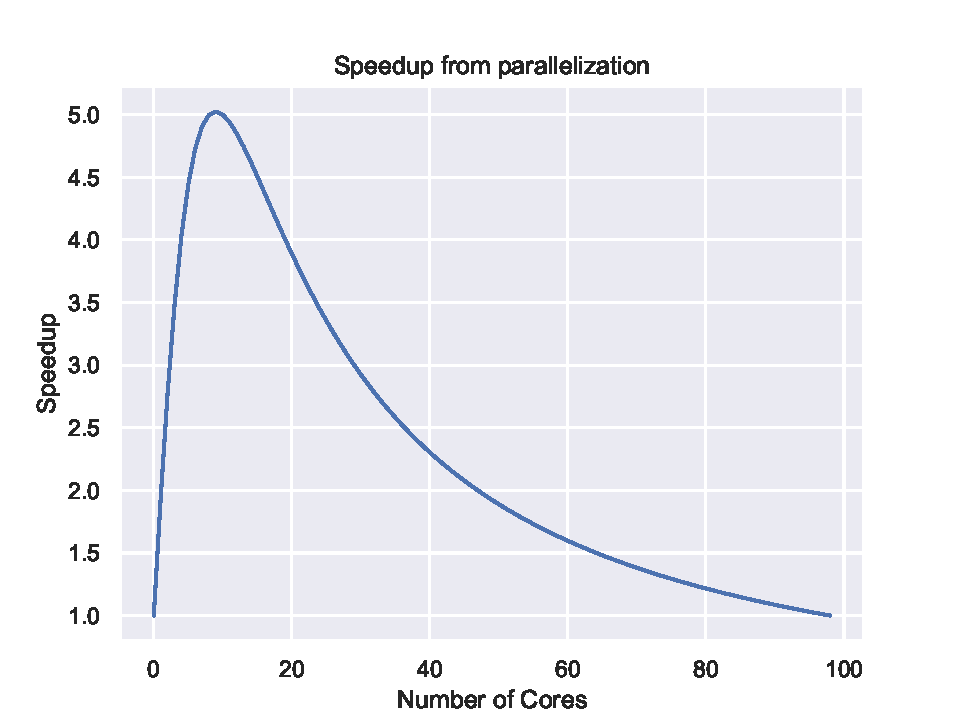
\includegraphics[width=\textwidth]{parallelization_plots/parallelization_speedup.pdf}
    \caption{Change of speedup in dependence of number of cores for $O_c = 0.01n$.}
    \label{fig:par_speed_001}
  \end{minipage}
  \hfill
  \begin{minipage}[t]{0.45\textwidth}
    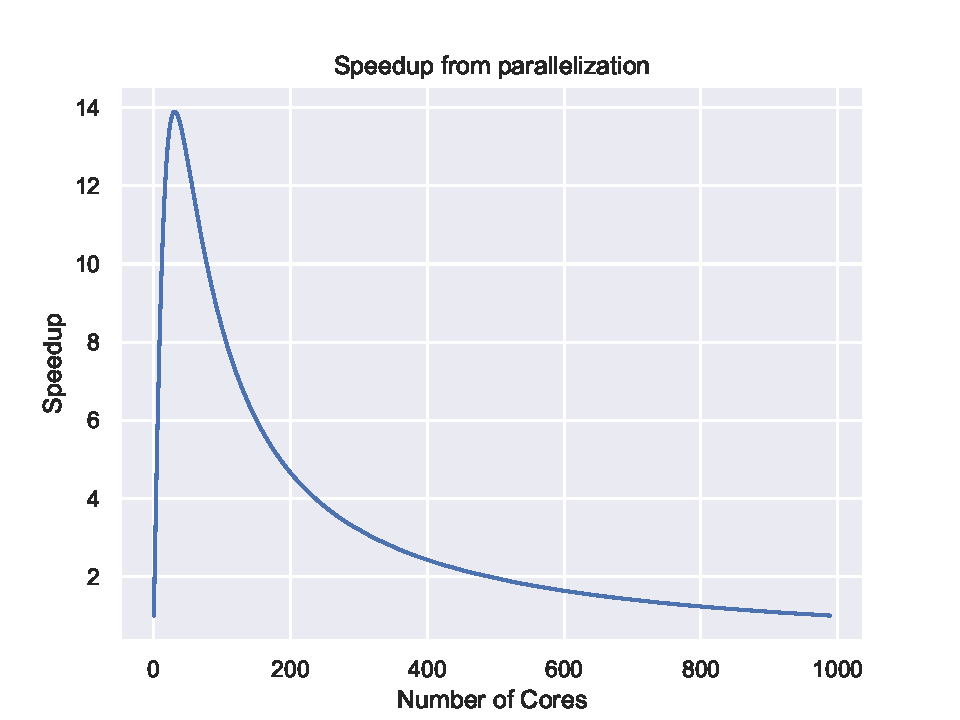
\includegraphics[width=1\textwidth]{parallelization_plots/parallelization_speedup_0001.pdf}
    \caption{Change of speedup in dependence of number of cores for $O_c = 0.001n$.}
    \label{fig:par_speed_0001}
  \end{minipage}
\end{figure}

\item
The total execution time is $T(n) = 10t_1 + \frac{1000}{n}t_1$. For $n = 10$ cores, the execution time is $T(10) = 10t_1 + 100t_1 = 110t_1$. The speedup gained from the parallelization is $S(10) = \frac{T_s)}{T_p(10)} = \frac{1010t_1}{110t_1} \approx 9.18$.

We assume the word "more" means additional and not a redistribution over the $1000t_1$ in the problem statement, therefore, the total number of parallizable operations becomes $\ge 1000$. For a load of $1.5$ and $3$ on one core we have the following speedups respectively:

\begin{equation}
\begin{split}
    S = \frac{1060t_1}{10t_1 + 150t_1} \approx 6.63 \\
    S = \frac{1210t_1}{10t_1 + 300t_1} \approx 3.90
\end{split}
\end{equation}

\end{enumerate}

\newpage

\section{Linear Algebra Operations}
\begin{enumerate}[a)]
\setcounter{enumi}{0}
\item
The row-major implementation is faster because we have better memory access patterns. This only comes into effect after a certain size of the matrix. The gap between the row-major and column-major implementation becomes bigger as the dimension $N \times N$ of the matrix increases. For one we can optimize the row-major implementation and save constants in the outer loop, secondly we also have more cache hits thanks to the better access pattern. Noticeable is that there is a jump around $512 \times 512$, which is where our problem doesn't fit fully into the (L3) cache anymore. 

\begin{figure}[h]
  \centering
  \begin{minipage}[t]{0.8\textwidth}
    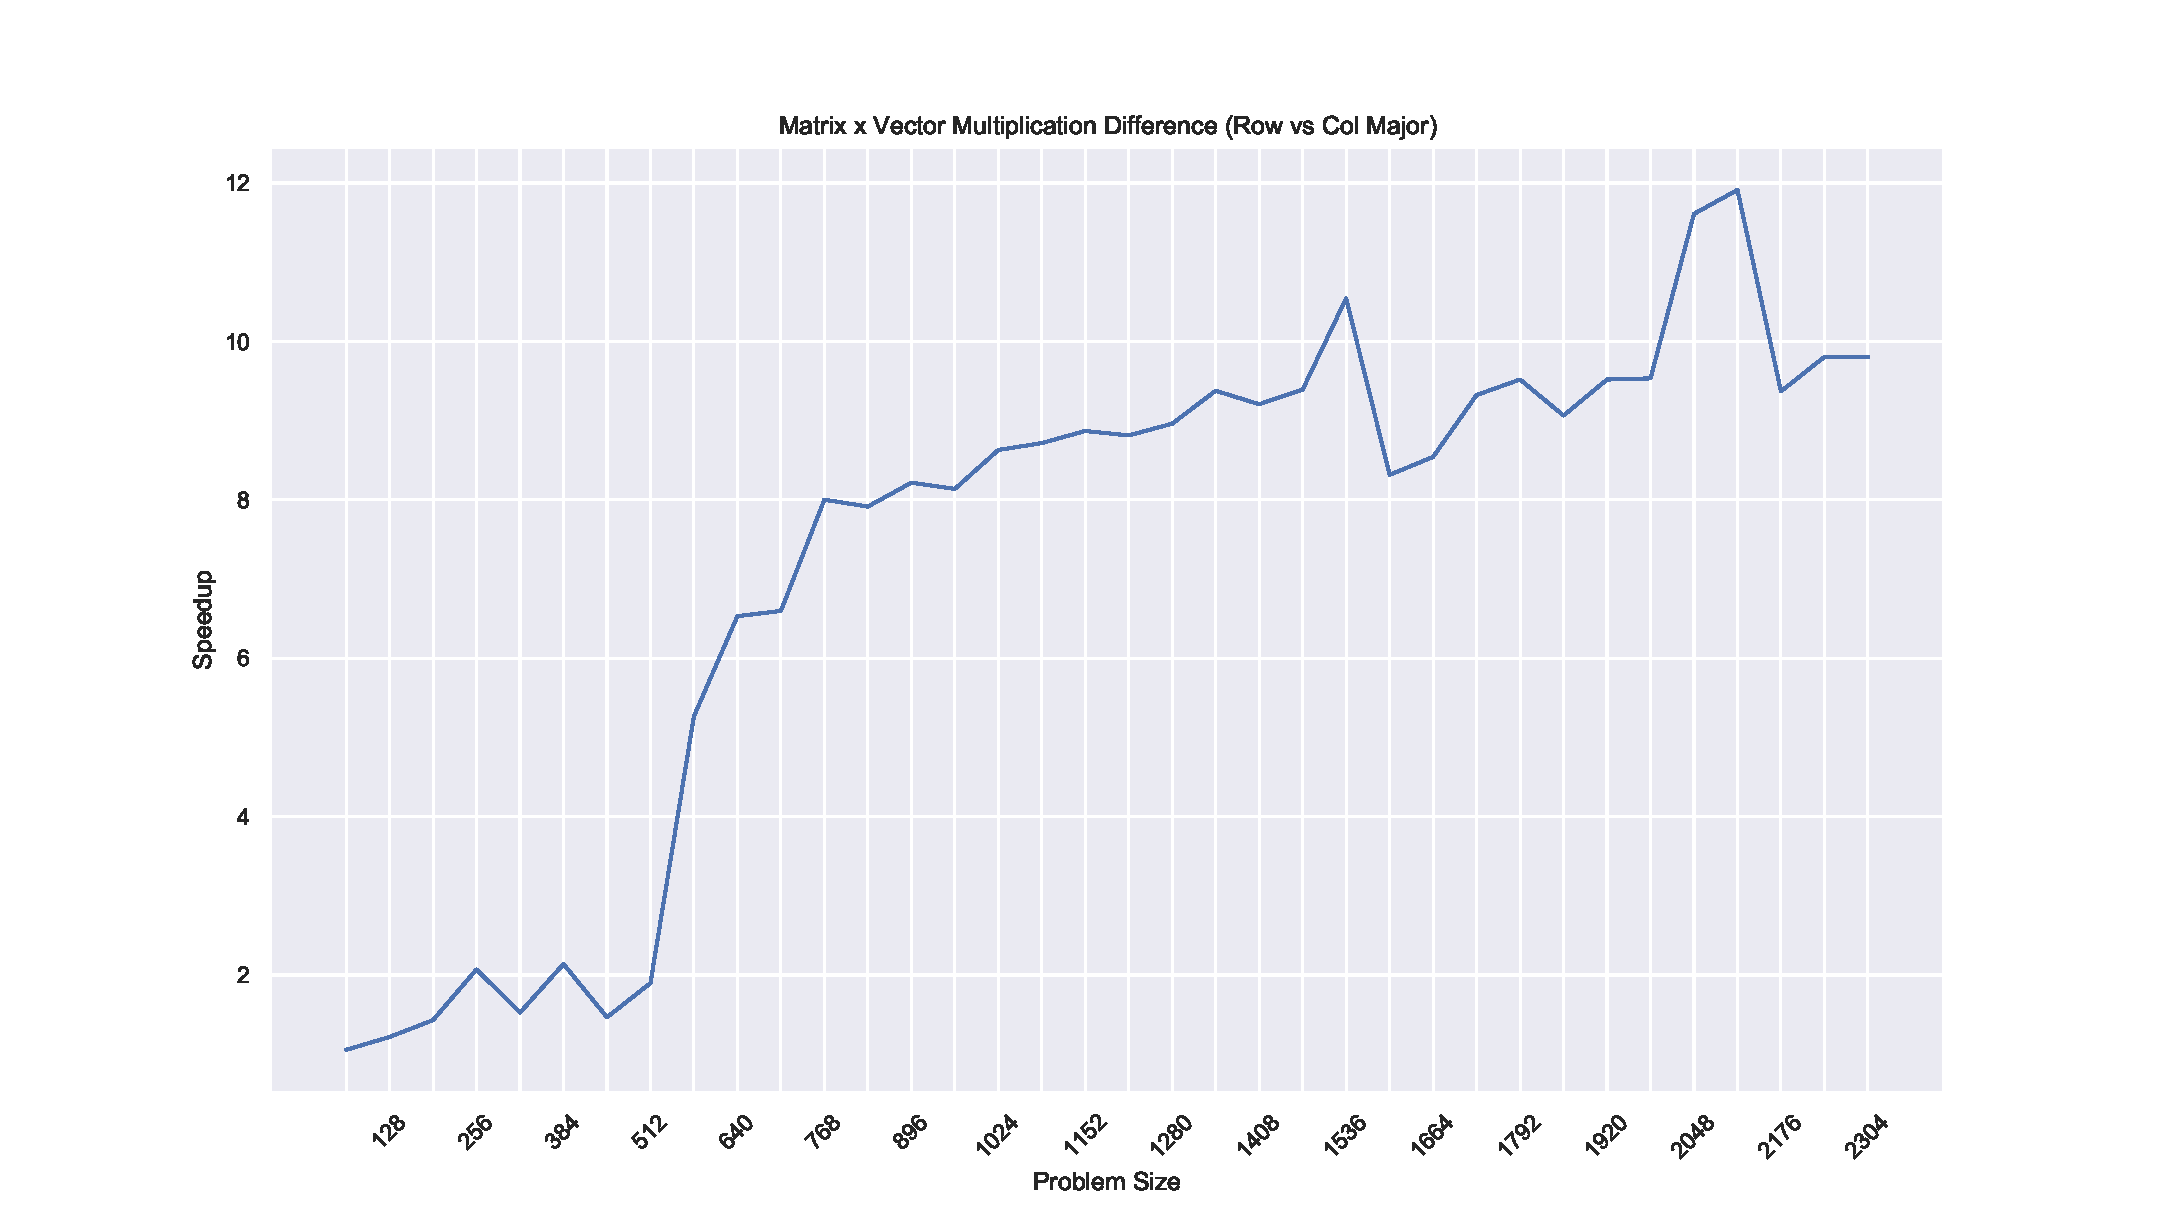
\includegraphics[width=\textwidth]{caching_plots/speedup_col_row.pdf}
    \caption{Speedup of row major versus column major implementation for matrix $\times$ vector multiplication.}
    \label{fig:speed_col_row}
  \end{minipage}
\end{figure}

\item
When running the matrix transpose we see that there is an optimal block size, namely size $8$. If we choose smaller or bigger blocks than that, we'll have worse performance. The performance of the different block sizes can be seen in Figure \ref{fig:mat_transpose}. The result is not surprising, as storing the blocks of size $8$ in the cache will use $2*8^2 * sizeof(double)$ space, which is $1$ KiB. Even though a bigger block size would still fit in cache, we assume that the reason this block size is better in performance is because of the compiler optimizations (we compile with $-O3$), like prefetching.

\begin{figure}[]
  \centering
  \begin{minipage}[t]{0.8\textwidth}
    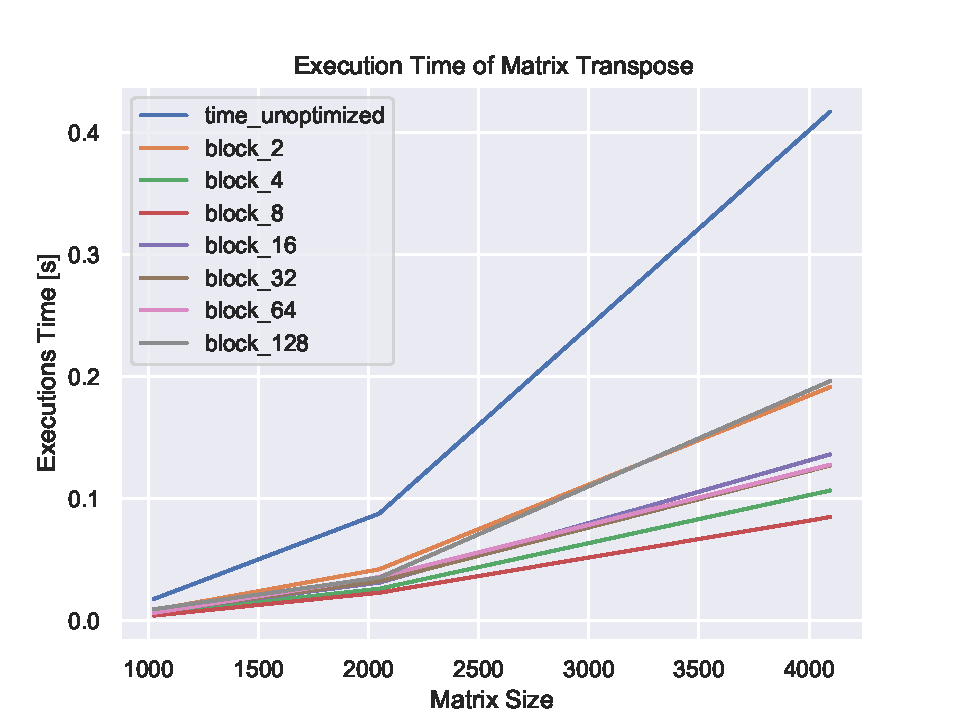
\includegraphics[width=\textwidth]{caching_plots/matrix_transpose.pdf}
    \caption{Execution time of matrix transpose for naive transpose and matrix blocks of various sizes. Measurements are taken for matrix sizes $1024$, $2048$ and $4096$.}
    \label{fig:mat_transpose}
  \end{minipage}
\end{figure}

\item
When running the matrix matrix multiplication we see that there is an optimal block size, namely size $16$. If we choose smaller or bigger blocks than that, we'll have worse performance. The performance of the different block sizes can be seen in Figure \ref{fig:mat_mat_mul}. The result is not surprising, as storing the blocks of size $8$ in the cache will use $3*16^2 * sizeof(double)$ space, which is $\approx 6$ KiB. Even though a bigger block size would still fit in cache, we assume that the reason this block size is better in performance is because of the compiler optimizations (we compile with $-O3$), like prefetching. As we expected, there is an increase in performance when we store the second matrix in column-major instead of row-major. The advantage of this is that we can then access the matrix elements as contiguous memory. This leads to better access patterns for the cache and therefore fewer cache-misses compared to the naive implementation or the regular block matrix matrix multiplication.

\begin{figure}[]
  \centering
  \begin{minipage}[t]{0.8\textwidth}
    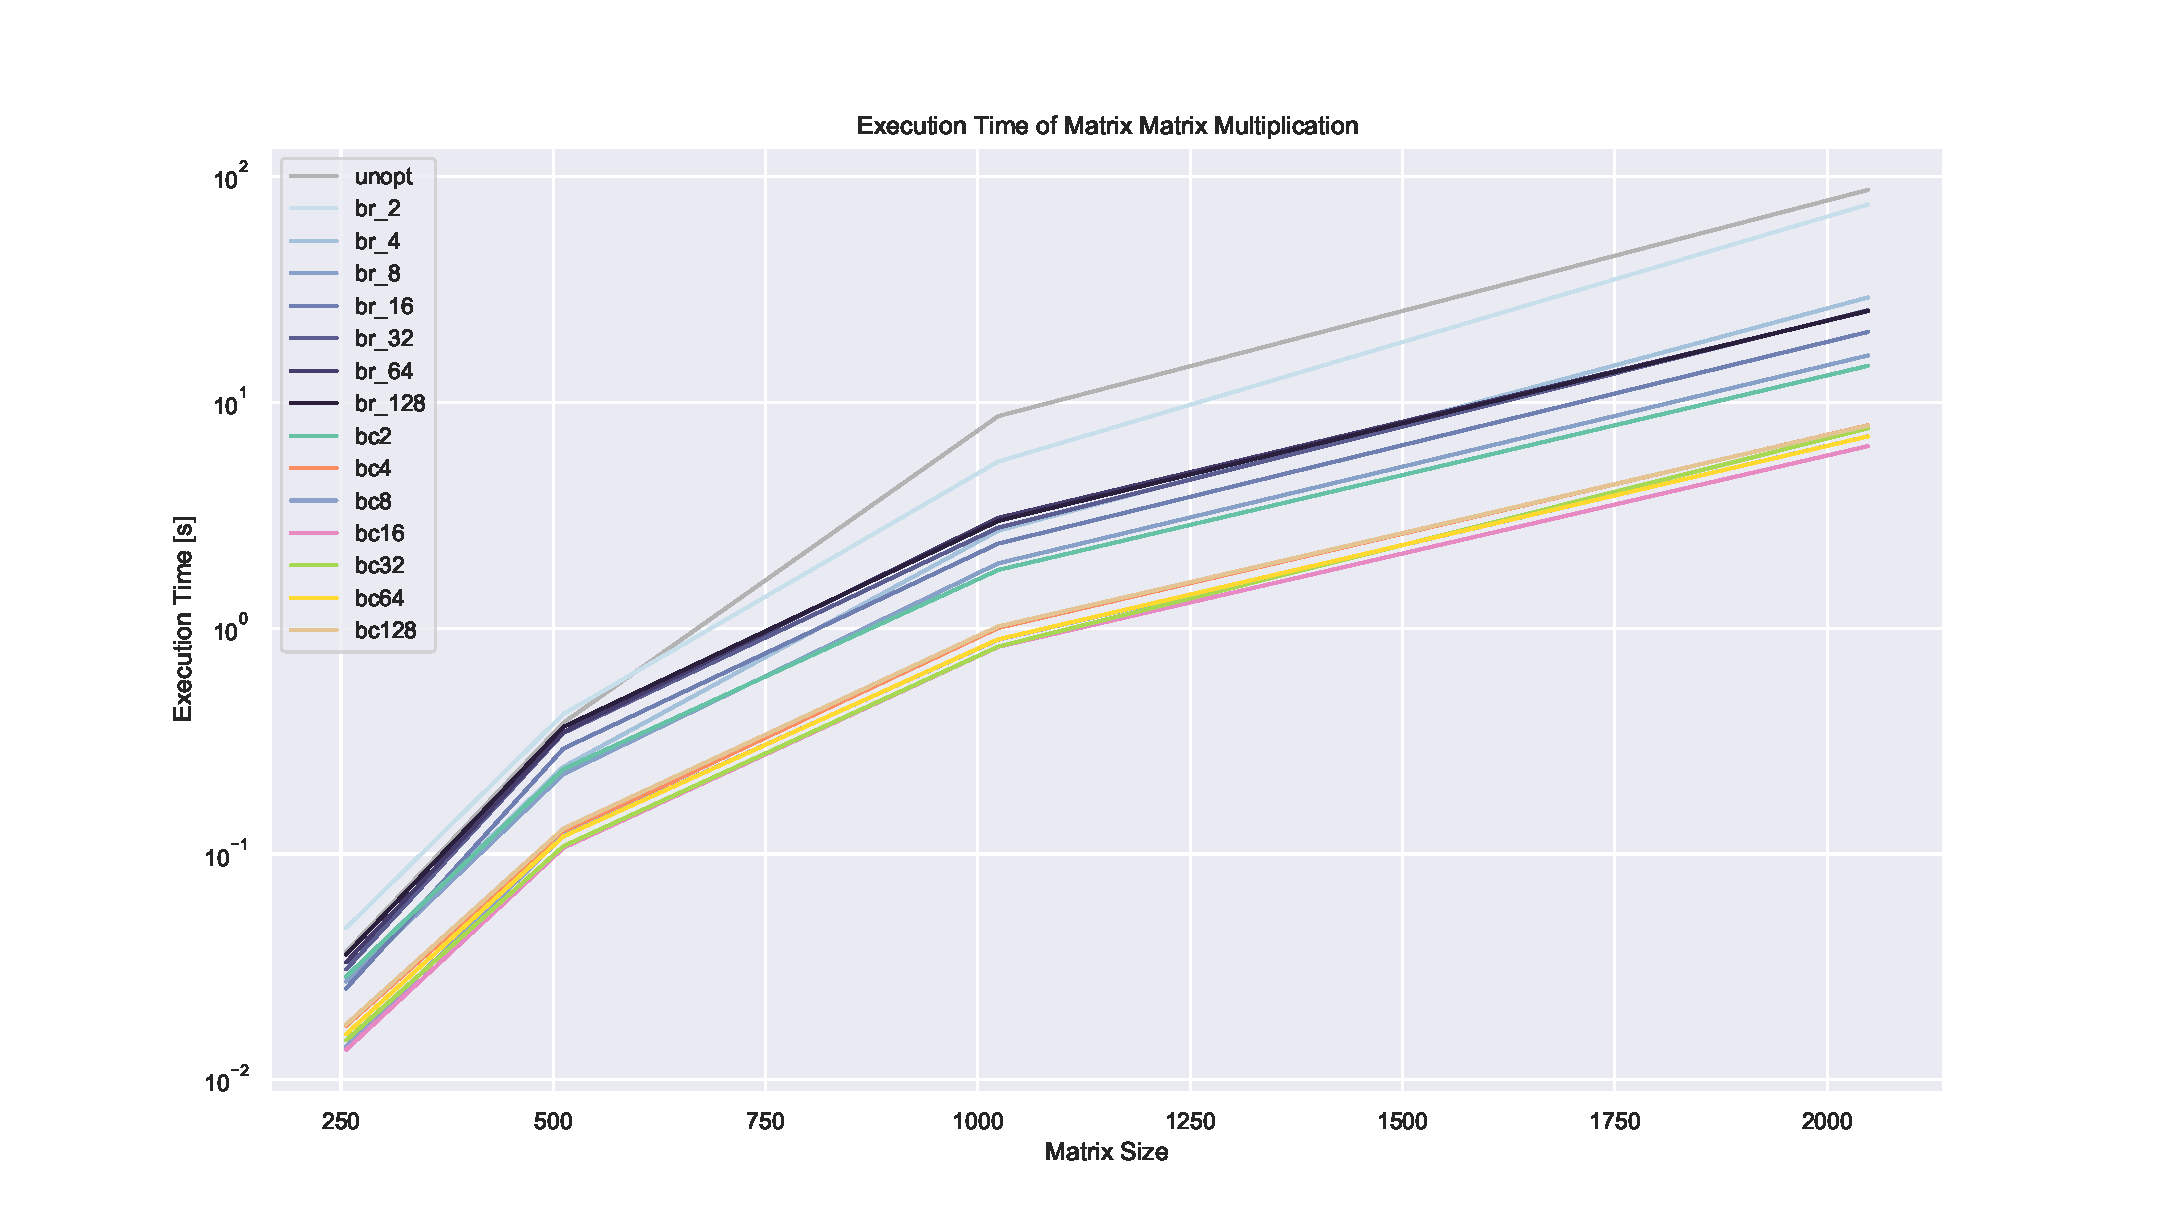
\includegraphics[width=\textwidth]{caching_plots/matrix_matrix.pdf}
    \caption{Execution time of matrix matrix multiplication for naive multiplication and matrix blocks of various sizes. $unopt$ is the measurement for the naive implementation, $bc$ are measurements for $A*B^T$, and $br$ are measurements for $A*B$. Measurements are taken for matrix sizes $256$, $512$, $1024$ and $2048$.}
    \label{fig:mat_mat_mul}
  \end{minipage}
\end{figure}

\end{enumerate}
\newpage 
 
\section{Cache size and cache speed}

Running the command from the exercise sheet on the Euler login node we find the cache sizes of the CPU, which are listed in Table \ref{table:1}.
{\begin{table}[h!]
 \centering
{\begin{tabular}{r r r}
    \toprule
    Cache & Size & Coherency Line Size \\
    \midrule
    L1 & 32KB & 64 \\
    L2 & 256KB & 64 \\
    L3 & 6144KB & 64 \\
    \bottomrule
\end{tabular}}
{\caption{Cache sizes and cache line size on Euler login node. Note that the L1 is twice the size, as there is one L1 cache for data and one for instructions.}    
\label{table:1}}
\end{table}}

When running our program for the different array access patterns, we get the operations per second shown in Figures \ref{fig:cache_o0} and \ref{fig:cache_o3}. For the code compiled with $-O3$ it is noticeable that the random access has a "burn-in" phase, as we don't have any cache prefetching and start (presumably) with a cold cache. The behaviour when our array gets big in size seems very random and the only distinct trend we notice is that the number of operations decreases steadily for the sequential accesses. In the case of $-O0$ we have a more stable picture. The $4$ byte strided access and the random access are both roughly equal over time and have a slight decrease in operations per second as the array size increases. There is not a very significant drop when the array size passes over a cache size and we have a smooth transition. We assume this is because for the bigger size we can still prefetch cachelines, which means that there will be a slightly higher fetching time, as we are in a higher level cache or in RAM, but mostly the operations will still have the same time as we have a lot of cache hits. The two methods are comparable, as we're frequently making cache hits with the random method. The $64$ byte strided access has the expected sudden drops in performance when we exceed the sizes of the cache levels, so it is a sharp transition. The reason for this is that we have to fetch a new cache line every time we do an operation, so the increase in cache line fetching time will lead to an overall worse operations per second performance. The drops match the cache sizes we found in \ref{table:1}. Foremost the change from the L1 to L2 and L3 to RAM have large gaps as when our array doesn't fit in the according memory anymore. For very large $N$ the random access will become continuously worse as we will get less cache hits. The same holds for the $64$ byte strided access, as the bigger our array gets, the more memory we need and henceforth also will save our data in higher level memory. This will lead to worse performance as we need to search further in the memory hierarchy until we find our data.

\begin{figure}[h]
  \centering
  \begin{minipage}[t]{0.45\textwidth}
    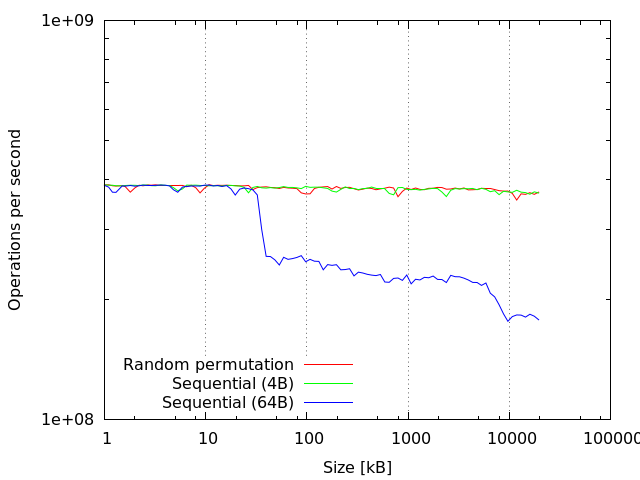
\includegraphics[width=\textwidth]{caching_plots/cache_access_O0.png}
    \caption{Number of operations for the three different access patterns on the Euler cluster in dependence of the array size. Compiler flag $-O0$.}
    \label{fig:cache_o0}
  \end{minipage}
  \hfill
  \begin{minipage}[t]{0.45\textwidth}
    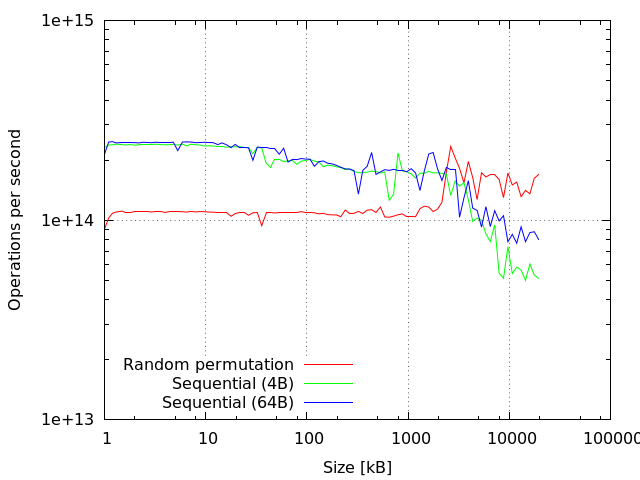
\includegraphics[width=1\textwidth]{caching_plots/cache_access_O3.png}
    \caption{Number of operations for the three different access patterns on the Euler cluster in dependence of the array size. Compiler flag $-O3$.}
    \label{fig:cache_o3}
  \end{minipage}
\end{figure}

\bigskip
%----------------------------------------------------------------------------------------
%	REFERENCE LIST
%----------------------------------------------------------------------------------------

\printbibliography

%----------------------------------------------------------------------------------------

\end{document}

